% dye_spectrum.tex
% by Troy Hix, May 2005
%----------------------------------------------------------------------------
\begin{figure}
\center
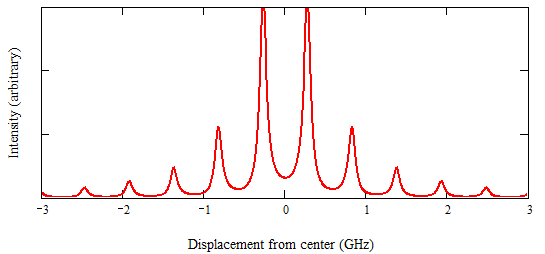
\includegraphics[width=6.00in]
{dye_spectrum/dye_spectrum.png}
\caption[Estimated dye laser spectrum]{Estimated dye laser spectrum. Each mode has a width of 50 MHz in a comb structure with a 550 MHz spacing. The comb is enveloped by a Lorentzian with a FWHM of 1 GHz. The dye laser subsystem, LambdaLok, stabilizes the envelope within 1 GHz of a specified wavelength setting. The comb structure may also slew underneath the 1 GHz envelope from shot to shot.}
\label{dye_spectrum}
\end{figure} 
%----------------------------------------------------------------------------
%----------------------------------------------------------------------------
%----------------------------------------------------------------------------


